\subsubsection{Pipeline B}

Pipeline B is concerned with finding the tip of the plant.
This is achieved by finding the highest point along the plant's stake which is covered by leaves.

For this purpose the longest vertical edge within an image is detected and it's lower point is
expected to be the plant's tip.

The following algorithm (or computational pipeline) has been developed in order to achieve this goal,
followed by a more formal description of the algorithm.

\begin{enumerate}
    \setlength{\itemsep}{0pt}
    \setlength{\parskip}{0pt}
    \item Edge detection to find contours
    \item Vertical blur to combine interrupted vertical lines (due to edge filter)
    \item High pass filter to create binary image of lines, this eliminates dots and short lines
    \item Count vertical line column-wise. Allow a horizontal tolerance window to accept slight slopes
    \item The lower point of the longest line is assumed to be plants stake
\end{enumerate}

The exact chosen algorithms have been gradually developed and refined by experimenting
based on images generated from the simulation or actual images from tomato plants.\\

\textbf{Edge detection:} There are plenty of edge detection algorithms to choose from but since
the final goal here only to locate vertical edges a simple and edge filter is sufficient, especially
it must must not find contours but find edges across color variations.

For this purpose the \textit{Sobel operator} has been chosen which is efficient and sufficient
for this purpose and combined with a high pass filter.
It uses two 3x3 kernels which are convoluted on the input image $I$ to approximate the horizontal
and vertical derivative at each pixel.\\

\noindent\begin{minipage}{.5\linewidth}
     \begin{equation}
         G_{x} = \begin{bmatrix}
                     +1 & 0 & -1\\
                     +2 & 0 & -2\\
                     +1 & 0 & -1
         \end{bmatrix} \ast I
     \end{equation}
\end{minipage}
\begin{minipage}{.5\linewidth}
    \begin{equation}
    G_{y} = \begin{bmatrix}
                +1 & +2 & +1\\
                0 &  0 &  0\\
                -1 & -2 & -1
    \end{bmatrix} \ast I
    \end{equation}
\end{minipage}\\

Which result in the x-coordinate as the increasing \textit{right} direction and y-coordinate as
increasing \textit{down} direction.
The gradient magnitude and direction can be calculated as follows:

\noindent\begin{minipage}{.5\linewidth}
             \begin{equation}
                 G = \sqrt{G_{x}^{2} + G_{y}^{2}}
             \end{equation}
\end{minipage}
\begin{minipage}{.5\linewidth}
    \begin{equation}
        \Theta = atan\left(\frac{G_{y}}{G_{x}}\right)
    \end{equation}
\end{minipage}\\

These values are in the implementation combined with a range check and low pass filter to better results:

\lstinputlisting[language={[Sharp]C}, caption = Edge dectection]{members/ssr/code/edge.cs}\vspace{5pt}

\textbf{Vertical Blur:} This applies just repeatedly a vertical average blur:
\begin{equation}
    \frac{1}{3}\begin{bmatrix}
        1 & 1 & 1
    \end{bmatrix}^{T}
\end{equation}

\textbf{High pass:} Only grey values below a certain threshold, which leads to removal of irrelevant
smaller dots and lines, see figure \ref{fig:v:3}\\

\textbf{Finding longest vertical edge:} At this point only a binary black and white image has remained.
Finding the longest vertical edge is conducted by preparing a boolean matrix in multiple steps.
Firstly, for every pixel a horizontal interpolation of adjacent horizontal pixels, along a variable
window is applied. This allows to include lines with a slight slope.

\lstinputlisting[language={[Sharp]C}, caption = Interpolate each pixel horizontally]{members/ssr/code/hinterpolate.cs}\vspace{5pt}

Now a boolean matrix has been constructed which is column-wise traversed to the longest sequence of true
values (longest vertical interpolated line):

\lstinputlisting[language={[Sharp]C}, caption = Find longest vertical boolean sequence]{members/ssr/code/vline.cs}\vspace{5pt}

The following figure shows the result of each step with the final results.

\begin{figure}[H]
    \centering
    \begin{minipage}[t]{0.24\textwidth}
        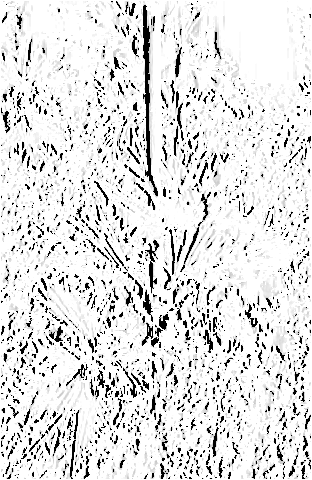
\includegraphics[width=\textwidth]{implementation/v-1.png}
        \caption{Sobel operator}
        \label{fig:v:1}
    \end{minipage}
    \hfill
    \begin{minipage}[t]{0.24\textwidth}
        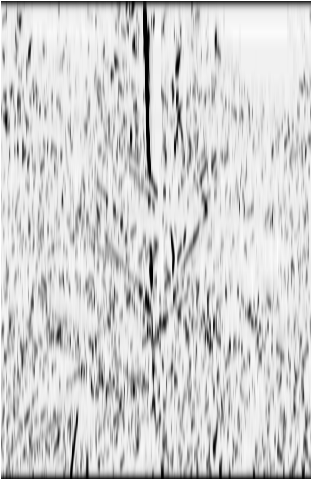
\includegraphics[width=\textwidth]{implementation/v-2.png}
        \caption{Vertical blur}
        \label{fig:v:2}
    \end{minipage}
    \hfill
    \begin{minipage}[t]{0.24\textwidth}
        \frame{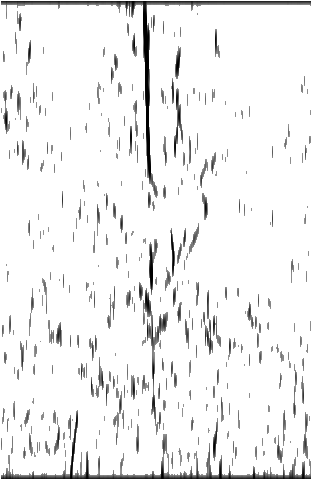
\includegraphics[width=\textwidth]{implementation/v-3.png}}
        \caption{High pass}
        \label{fig:v:3}
    \end{minipage}
    \hfill
    \begin{minipage}[t]{0.24\textwidth}
        \frame{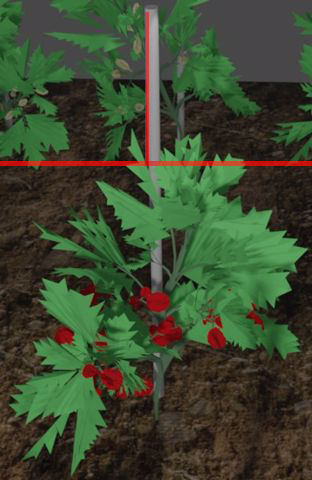
\includegraphics[width=\textwidth]{implementation/v-4.png}}
        \caption{Detection plant tip}
        \label{fig:v:4}
    \end{minipage}
\end{figure}